\documentclass[11pt,a4paper]{article}
\usepackage[utf8]{inputenc}
\usepackage[english]{babel}
\usepackage[left=2.5cm, right=2.5cm, top=2.5cm, bottom=2.5cm]{geometry}
\usepackage{hyperref}
\usepackage{graphicx}
\usepackage{times}
\usepackage[bottom]{footmisc}
\usepackage{listings}
\usepackage{bm}
\usepackage{amsmath}
\usepackage{algpseudocode}
\usepackage{algorithm}
\usepackage{titlesec}
\usepackage{tikz}
\usepackage{tikz-qtree}

\titleformat{\subsubsection}[runin]{}{}{}{}[]

\title{\textbf{Advanced Machine Learning -- Homework 3}}
\author{Anna Berger, Ashwin Sadananda Bhat (AML 25)}

\setlength{\parindent}{0pt}

\usepackage{booktabs}

\begin{document}
\maketitle
  
 \section*{Exercise 1}
 To investigate the effect of dimensionality reduction and PCA we apply the Bayesian approach to the predict whether a person has breast cancer or not. There are two possible classes: benign (labelled as 2) and malicious (labelled as 4). In the assignment we refer to them as B and M respectively.
 
  From the data we can estimate the prior distributions of these classes by counting the number of B's and M's and normalising them by the total number of people: $$ priors \approx (0.65, 0.35) $$ 
 
 Hereafter we define the error as the ratio of misclassified objects.
 
 
 \subsection*{Part a}
 
 \begin{enumerate}
	 \item \textbf{Univariate classifiers}
	\begin{enumerate}
		\item \textbf {x2 (Clump Thickness) only} \\
		In this case, the feature is the second column of the dataset which represents clump thickness.
		First, we estimate the mean and the variance of this feature for each class:
		$$\bar{x}_{2B} \approx 2.936, \quad var(x_{2B}) \approx 2.739, $$
		$$\bar{x}_{2M} \approx 7.133, \quad var(x_{2M}) \approx 6.215.$$
		
		Then we fit the Gaussians using these estimations and apply the Bayes rule to classify objects.
		The statistics for this classifier can be seen from the Table \ref{tab:results-x2}:
		
		\begin{table}[H]
			\centering
				\begin{tabular}{lrr}
					\toprule
					 & \textbf{Train} & \textbf{Validation}  \\ \midrule
					Error & 0.137 & 0.146 \\	
					Precision (malicious) & 0.907 &0.868 \\
					Recall (malicious) & 0.678 & 0.6875 \\
					\bottomrule
				\end{tabular}
			\caption{Univariate classifier (feature x2).}
			\label{tab:results-x2}
		\end{table}
		
		The confusion matrices for train and validation sets are shown in the Figures \ref{fig:conf_train_x2.png} and \ref{fig:conf_val_x2.png}.
		
		\begin{figure}[H]\centering
				\begin{minipage}{0.49\textwidth}
					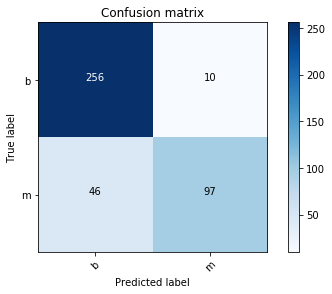
\includegraphics[width=\linewidth]{figures/conf_train_x2.png}
					\caption{Feature x2, train}\label{fig:conf_train_x2.png}
				\end{minipage}
				\begin{minipage}{0.49\textwidth}
 				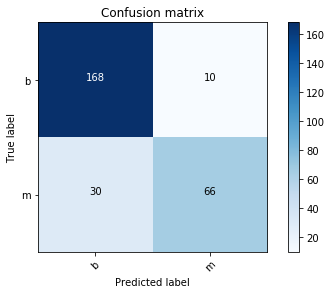
\includegraphics[width=\linewidth]{figures/conf_val_x2.png}
				\caption{Feature x2, val}\label{fig:conf_val_x2.png}
			\end{minipage}
		\end{figure}

	\item \textbf {First principal component} \\
	We perform SVD on the covariance matrix for the total dataset and obtain eigenvalues (diagonal matrix $s$) and eigenvectors for it (columns of matrix $U$). The first column of matrix $U$ is the first principal component which covers 68,7\% of the variance of the dataset and looks as follows:
	$$ [-0.3059, -0.4085, -0.3859, -0.3280 , -0.2293, -0.4522, -0.2830 , -0.3581, -0.1329]^\tau $$
	
	Then, we project all the datapoints on the obtained vector.
	
	After that, we estimate the mean and the variance of projected dataset:
	$$\bar{x}_{pca1B} \approx -4.718, \quad var(x_{pca1B}) \approx 3.566, $$
	$$\bar{x}_{pca1M} \approx -17.729, \quad var(x_{pca1M}) \approx 19.710.$$
	
	Then we fit the Gaussians using these estimations and apply the Bayes rule to classify objects.
	The statistics for this classifier can be seen from the Table \ref{tab:results-pca-1}:
	
	\begin{table}[H]
		\centering
		\begin{tabular}{lrr}
			\toprule
			& \textbf{Train} & \textbf{Validation}  \\ \midrule
			Error & 0.037 & 0.014 \\	
			Precision (malicious) & 0.932 & 0.969 \\
			Recall (malicious) & 0.965 & 0.989 \\
			\bottomrule
		\end{tabular}
		\caption{Univariate classifier (first principal component).}
		\label{tab:results-pca-1}
	\end{table}
	
	The confusion matrices for train and validation sets are shown in the Figures \ref{fig:conf_train_pca_1.png} and \ref{fig:conf_val_pca_1.png}.
	
	\begin{figure}[H]\centering
		\begin{minipage}{0.49\textwidth}
			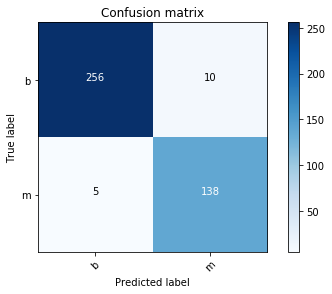
\includegraphics[width=\linewidth]{figures/conf_train_pca_1.png}
			\caption{The first principal component, train set}\label{fig:conf_train_pca_1.png}
		\end{minipage}
		\begin{minipage}{0.49\textwidth}
		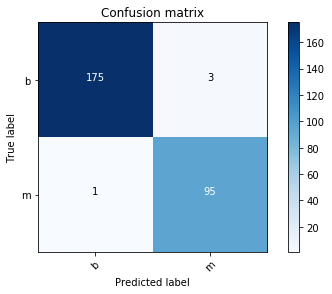
\includegraphics[width=\linewidth]{figures/conf_val_pca_1.png}
		\caption{The first principal component, val set}\label{fig:conf_val_pca_1.png}
		\end{minipage}
	\end{figure}		
		
	\end{enumerate}

	\item \textbf{Bivariate classifiers}
	\begin{enumerate}
		\item \textbf {x2 and x7 (Clump Thickness and Bare Nuclei)} \\
		In this case, the features are the second and the seventh columns of the dataset which represent clump thickness and bare nuclei.
		
		First, we estimate the mean and the covariance of this feature for each class:
		\[
		\bar{x}_{27B} \approx (2.936,  1.365), \quad 
		\Sigma_{27B} \approx 
		\begin{bmatrix}
		2.739 & 0.220   \\
		0.220 & 1.470   \\
		\end{bmatrix}.
		\]
		
		\[
		\bar{x}_{27M} \approx (7.133,  7.706), \quad 
		\Sigma_{27M} \approx 
		\begin{bmatrix}
		6.215 & 0.082   \\
		0.082 & 9.082   \\
		\end{bmatrix}.
		\]
		
		Then we fit the Gaussians using these estimations and apply the Bayes rule to classify objects.
		The statistics for this classifier can be seen from the Table \ref{tab:results-x2-x7}:
		
		\begin{table}[H]
			\centering
			\begin{tabular}{lrr}
				\toprule
				& \textbf{Train} & \textbf{Validation}  \\ \midrule
				Error & 0.059 & 0.054 \\	
				Precision (malicious) & 0.916 &0.918 \\
				Recall (malicious) & 0.916 & 0.927 \\
				\bottomrule
			\end{tabular}
			\caption{Bivariate classifier (features x2, x7).}
			\label{tab:results-x2-x7}
		\end{table}
		
		The confusion matrices for train and validation sets are shown in the Figures \ref{fig:conf_train_x2_x7.png} and \ref{fig:conf_val_x2_x7.png}.
		
		\begin{figure}[H]\centering
			\begin{minipage}{0.49\textwidth}
				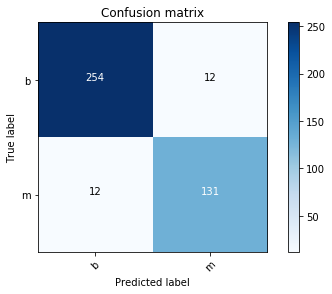
\includegraphics[width=\linewidth]{figures/conf_train_x2_x7.png}
				\caption{Features x2, x7, train}\label{fig:conf_train_x2_x7.png}
			\end{minipage}
			\begin{minipage}{0.49\textwidth}
				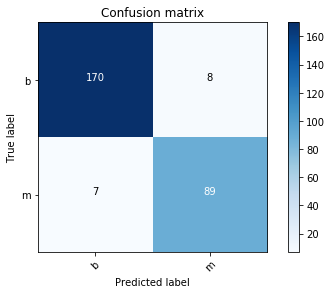
\includegraphics[width=\linewidth]{figures/conf_val_x2_x7.png}
				\caption{Features x2, x7, val}\label{fig:conf_val_x2_x7.png}
			\end{minipage}
		\end{figure}
		
	\item \textbf {First two principal components} \\
	Now we take first two columns of the matrix $U$ --- first two principal components. They cover 76.1\% of the variance of the dataset.
	The first principal component is already shown in a previous part, the second principal component is given by:
	 $$ [0.0756,  0.2158,  0.1710, -0.2682,  0.1916, -0.7441,  0.0371,  0.4670,  0.1917]^\tau$$
	
	 Then, we project all the datapoints on these vectors.
	
	After that, we estimate the mean and the covariance of projected dataset:
	
	\[
	\bar{x}_{pca12B} \approx (-4.718,  0.659), \quad 
	\Sigma_{pca12B} \approx 
	\begin{bmatrix}
	3.567 & -0.129   \\
	-0.129 & 0.932   \\
	\end{bmatrix}.
	\]
	
	\[
	\bar{x}_{pca12M} \approx (-17.729,  0.210), \quad 
	\Sigma_{pca12M} \approx 
	\begin{bmatrix}
	19.709 & -3.593  \\
	-3.593 & 12.923   \\
	\end{bmatrix}.
	\]
	
	
	Then we fit the Gaussians using these estimations and apply the Bayes rule to classify objects.

	
	\begin{table}[H]
		\centering
		\begin{tabular}{lrr}
			\toprule
			& \textbf{Train} & \textbf{Validation}  \\ \midrule
			Error & 0.037 & 0.021 \\	
			Precision (malicious) & 0.927 & 0.959 \\
			Recall (malicious) & 0.972 & 0.979 \\
			\bottomrule
		\end{tabular}
		\caption{Bivariate classifier (first two principal components).}
		\label{tab:results-pca-12}
	\end{table}
	
	The confusion matrices for train and validation sets are shown in the Figures \ref{fig:conf_train_pca_12.png} and \ref{fig:conf_val_pca_12.png}.
	
	\begin{figure}[H]\centering
		\begin{minipage}{0.49\textwidth}
			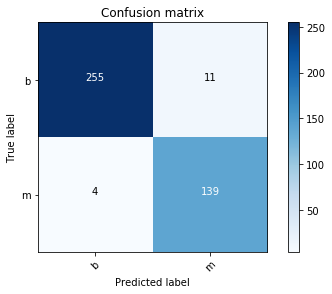
\includegraphics[width=\linewidth]{figures/conf_train_pca_12.png}
			\caption{First two principal components, train set}\label{fig:conf_train_pca_12.png}
		\end{minipage}
		\begin{minipage}{0.49\textwidth}
			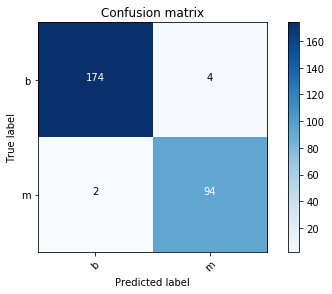
\includegraphics[width=\linewidth]{figures/conf_val_pca_12.png}
			\caption{First two principal components, val set}\label{fig:conf_val_pca_12.png}
		\end{minipage}
	\end{figure}	
	
		
	\end{enumerate}
	
	\item \textbf{Multivariate classifiers}
	\begin{enumerate}
		\item \textbf{The principal components which explain 80\% of the variance} \\
		We found out that the first three principal components cover 80\% of the variance of the whole dataset, precisely 82.3\%.
		The third principal component is given by:
		$$ [0.8107, -0.0523,  0.0440, -0.5190, -0.1229, 0.1079, -0.0952, -0.1489, -0.1033]^\tau $$
		
		We repeat the described procedure: project all the data points on the first three eigenvectors and estimate the mean and the covariance of projected dataset for both classes:
		
		\[
		\bar{x}_{pca123B} \approx (-4.718, 0.659,  1.059), \quad 
		\Sigma_{pca123B} \approx 
		\begin{bmatrix}
		3.567 & -0.129 & -0.635   \\
		-0.129 & 0.932 & 0.312  \\
		-0.635 & 0.312 & 1.691 \\
		\end{bmatrix}.
		\]
		
		\[
		\bar{x}_{pca123M} \approx (-17.729,  0.210, 1.437), \quad 
		\Sigma_{pca123M} \approx 
		\begin{bmatrix}
		19.709 & -3.593 & 4.411 \\
		-3.593 & 12.923 & -0.471   \\
		4.411 & -0.471 & 9.053 \\
		\end{bmatrix}.
		\]
		
		The statistics for this classifier can be seen from the Table \ref{tab:results-pca-123}:
		
		\begin{table}[H]
			\centering
			\begin{tabular}{lrr}
				\toprule
				& \textbf{Train} & \textbf{Validation}  \\ \midrule
				Error & 0.037 & 0.022 \\	
				Precision (malicious) & 0.921 & 0.959 \\
				Recall (malicious) & 0.979 & 0.979 \\
				\bottomrule
			\end{tabular}
			\caption{First three principal components.}
			\label{tab:results-pca-123}
		\end{table}
		
		The confusion matrices for train and validation sets are shown in the Figures \ref{fig:conf_train_pca_123.png} and \ref{fig:conf_val_pca_123.png}.
		
		\begin{figure}[H]\centering
			\begin{minipage}{0.49\linewidth}
				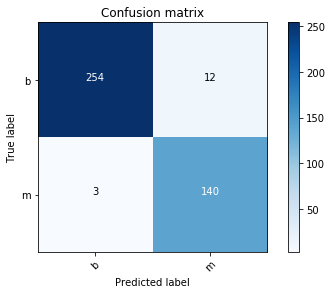
\includegraphics[width=\linewidth]{figures/conf_train_pca_123.png}
				\caption{First two principal components, train set}\label{fig:conf_train_pca_123.png}
			\end{minipage}
			\begin{minipage}{0.49\linewidth}
				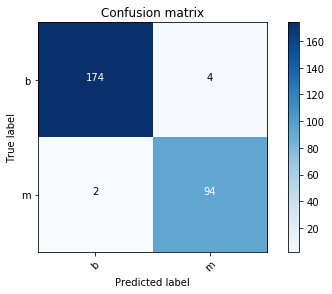
\includegraphics[width=\linewidth]{figures/conf_val_pca_123.png}
				\caption{First two principal components, val set}\label{fig:conf_val_pca_123.png}
			\end{minipage}
		\end{figure}	
		
		\item \textbf{All inputs} \\
		In this case the features are all the columns from the second to the tenth.
		We again estimate the mean and the covariance of the dataset (the number of dimensions is equal to 9, that's why we decided not to overload the report with the matrix 9x9), then fit the Gaussians for both classes and apply the Bayes rule to classify the objects.
		
		The statistics for this classifier can be seen from the Table \ref{tab:results-all}:
		
		\begin{table}[H]
			\centering
			\begin{tabular}{lrr}
				\toprule
				& \textbf{Train} & \textbf{Validation}  \\ \midrule
				Error & 0.048 & 0.033 \\	
				Precision (malicious) & 0.897 & 0.931 \\
				Recall (malicious) & 0.972 & 0.979 \\
				\bottomrule
			\end{tabular}
			\caption{Multivariate classifier (all inputs).}
			\label{tab:results-all}
		\end{table}
		
		The confusion matrices for train and validation sets are shown in the Figures \ref{fig:conf_train_all.png} and \ref{fig:conf_val_all.png}.
		
		\begin{figure}[H]\centering
			\begin{minipage}{0.49\linewidth}
				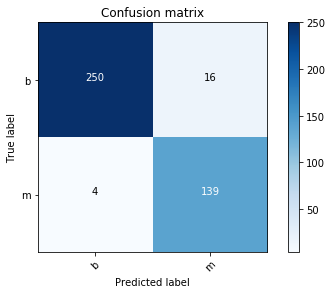
\includegraphics[width=\linewidth]{figures/conf_train_all.png}
				\caption{All inputs, train set}\label{fig:conf_train_all.png}
			\end{minipage}
			\begin{minipage}{0.49\linewidth}
				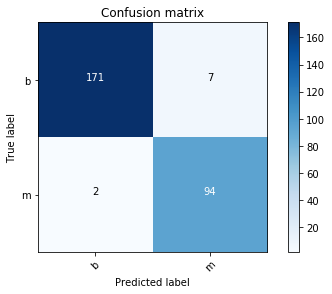
\includegraphics[width=\linewidth]{figures/conf_val_all.png}
				\caption{All inputs, val set}\label{fig:conf_val_all.png}
			\end{minipage}
		\end{figure}	
		
	\end{enumerate}
	
	\end{enumerate}

\subsection*{Part b}
In this exercise we explored several versions of the classifier. The univariate classifier using one raw feature from the data showed the worst performance, as it didn't contain enough information for good prediction. Moreover, it's always hard to choose the most representative feature manually. The bivariate classifier using two features performed much better, but it wasn't in the top according to validation error (and the problem of choosing the most representative pair of feature is even harder).

We obtained the lowest validation error on the validation set with the approach using the first principal component. We think it is a reasonable balance between a number of parameters to estimate (it is already enough to capture the patterns in the data and small enough to avoid overfitting to the training data). We got slightly bigger validation error with the first two and three principal components, however, we don't need to add more features as they don't improve the results.

In the task of cancer detection, recall for malicious class is extremely important. The best approach with the first principal component showed the best recall for the malicious class as well as the best precision for this class again proving that the first principal component covers the majority of important information in this dataset.

In the last experiment with all inputs, we saw that even using all raw features from the dataset, we can't achieve the same performance as when applying PCA to extract information from the data.

\section*{Exercise 2}
\subsection*{Part a}

In this exercise we apply the logistic classifier (the implementation from scikit-learn python library, namely LogisticRegression) to this problem. The regularization parameter (for l2 regularization) is set to 1.  Our training set consists of all provided features (9 columns). The adaptation of inputs (concatenation 1 as the first coordinate of inputs) and outputs (transformation from probabilities to labels 0 and 1) is done inside the algorithm provided by scikit-learn, so we don't have to do it manually.
 
The results for the logistic classifier can be seen from the Table \ref{tab:results-log}:

\begin{table}[H]
	\centering
	\begin{tabular}{lrr}
		\toprule
		& \textbf{Train} & \textbf{Validation}  \\ \midrule
		Error & 0.034 & 0.021 \\	
		Precision (malicious) & 0.957 & 0.978 \\
		Recall (malicious) & 0.944 & 0.958 \\
		\bottomrule
	\end{tabular}
	\caption{Logistic classifier (all inputs).}
	\label{tab:results-log}
\end{table}

The confusion matrices for train and validation sets are shown in the Figures \ref{fig:conf_train_log} and \ref{fig:conf_val_log}.

\begin{figure}[H]\centering
	\begin{minipage}{0.49\linewidth}
		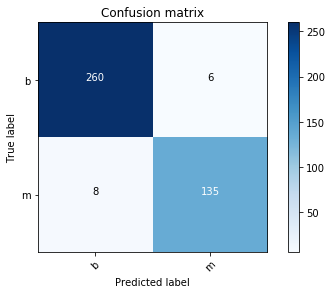
\includegraphics[width=\linewidth]{figures/conf_train_log.png}
		\caption{Logistic classifier, train set}\label{fig:conf_train_log}
	\end{minipage}
	\begin{minipage}{0.49\linewidth}
		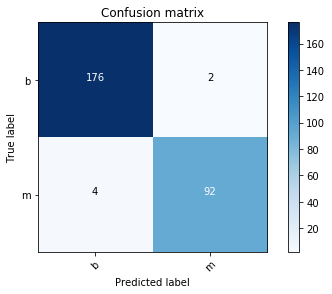
\includegraphics[width=\linewidth]{figures/conf_val_log.png}
		\caption{Logistic classifier, val set}\label{fig:conf_val_log}
	\end{minipage}
\end{figure}	

Logistic classifier achieves the same level of accuracy as the best approach from the previous exercise --- the approach with first two principal components obtained the lowest error 0.021 on the validation set. However, the recall on the validation set is slightly higher for the Bayesian approach with the first two principal components and we suppose that recall for malicious class is essential for the problem of cancer detection.

\subsection*{Part b}
In Exercise 3 we used a generative approach to classify the objects: we explicitly modelled the distributions of classes $p(x| B)$ and $p(x | M)$ to determine class-conditional densities for each class individually. To get posterior probabilities, we applied Bayes theorem. Having found posterior probabilities, we used decision theory to determine class membership for each new input. It is rather demanding approach in which one need to estimate a lot of parameters $\left(n + \frac{n(n + 1)}{2}\right)$илиля  in this particular case, where $n$ is the number of features), therefore, we need a large training set. However, it can be useful when we need to sample new datapoints from the distribution.

In Exercise 4 we used discriminative approach to modelling: we first determined the posterior class probabilities $p(B | x)$ and $p(M | x)$ and then used standard decision theory to assign each new input its category. The advantage of this approach is that it is less computationally expensive and requires less parameters to estimate, which may lead to a better predictive performance (especially under the lack of data conditions). On the other hand, by using this approach, we lose some information about structure of density probabilities.

 
\end{document}

